\chapter{DP Simulation}


\TODO{
    Give an overview of DP systems. Should not go too far into the details of how it is modelled, but enough to give
    an overview of the systems characteristics.

    Things to do:\\
        - Global system overview \\
        - Identify global system as being non-linear, causal, time invarient and dynamic\\
    
}

A dynamic positioning system is a system on board a ship that controls the ship's actuators such that the position of
the ship is kept constant, thus counteracting environmental forces \parencite{duDynamicPositioningShips2018}. This
allows ships to perform operations such as pipe-laying or construction in places where the waterdepth would otherwise be
restricting. A DP vessel can also reposition much faster than a ship operating on anchors
\parencite{aiModelingSimulationDeepwater2018}.

This chapter will describe the main components of a DP system and outline the mathematical properties of the system.

\section{DP System}
This section will describe the main components that make up a DP system. A global overview will be given and each
individual section will be futher explained.

Overall, most dynamic positioning systems have a similiar structure. The main components are the reference system,
observer, controller and thrusters.

\begin{figure}
    \centering
    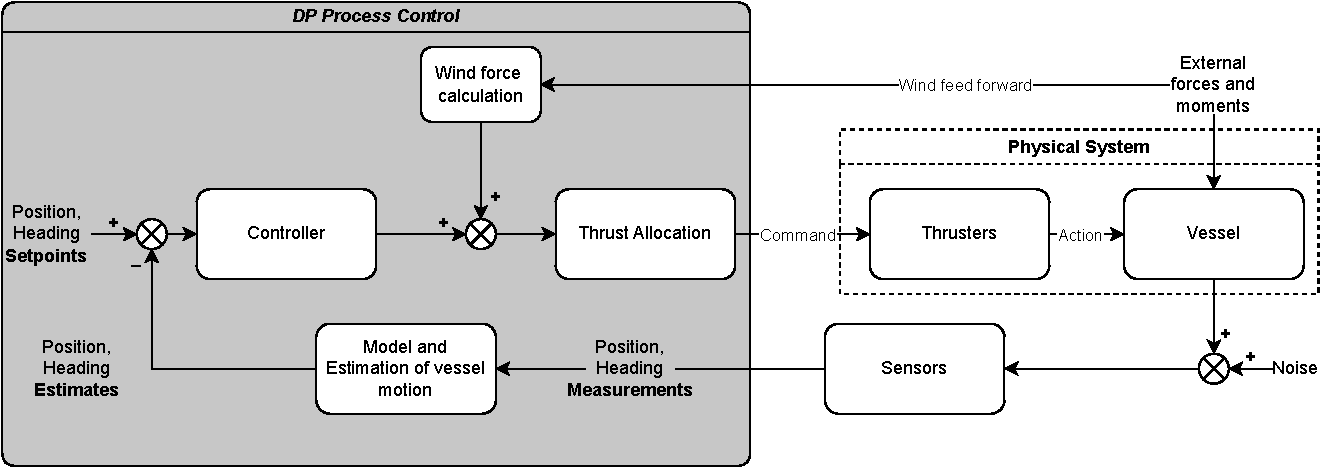
\includegraphics[width=0.75\linewidth]{report/images/diagrams/DP_overview.pdf}
    \caption{Overview of DP system components}
    \label{fig:dp_overview}
\end{figure}



